\documentclass{standalone}
\usepackage{tikz}
\usetikzlibrary{patterns, positioning}


\begin{document}
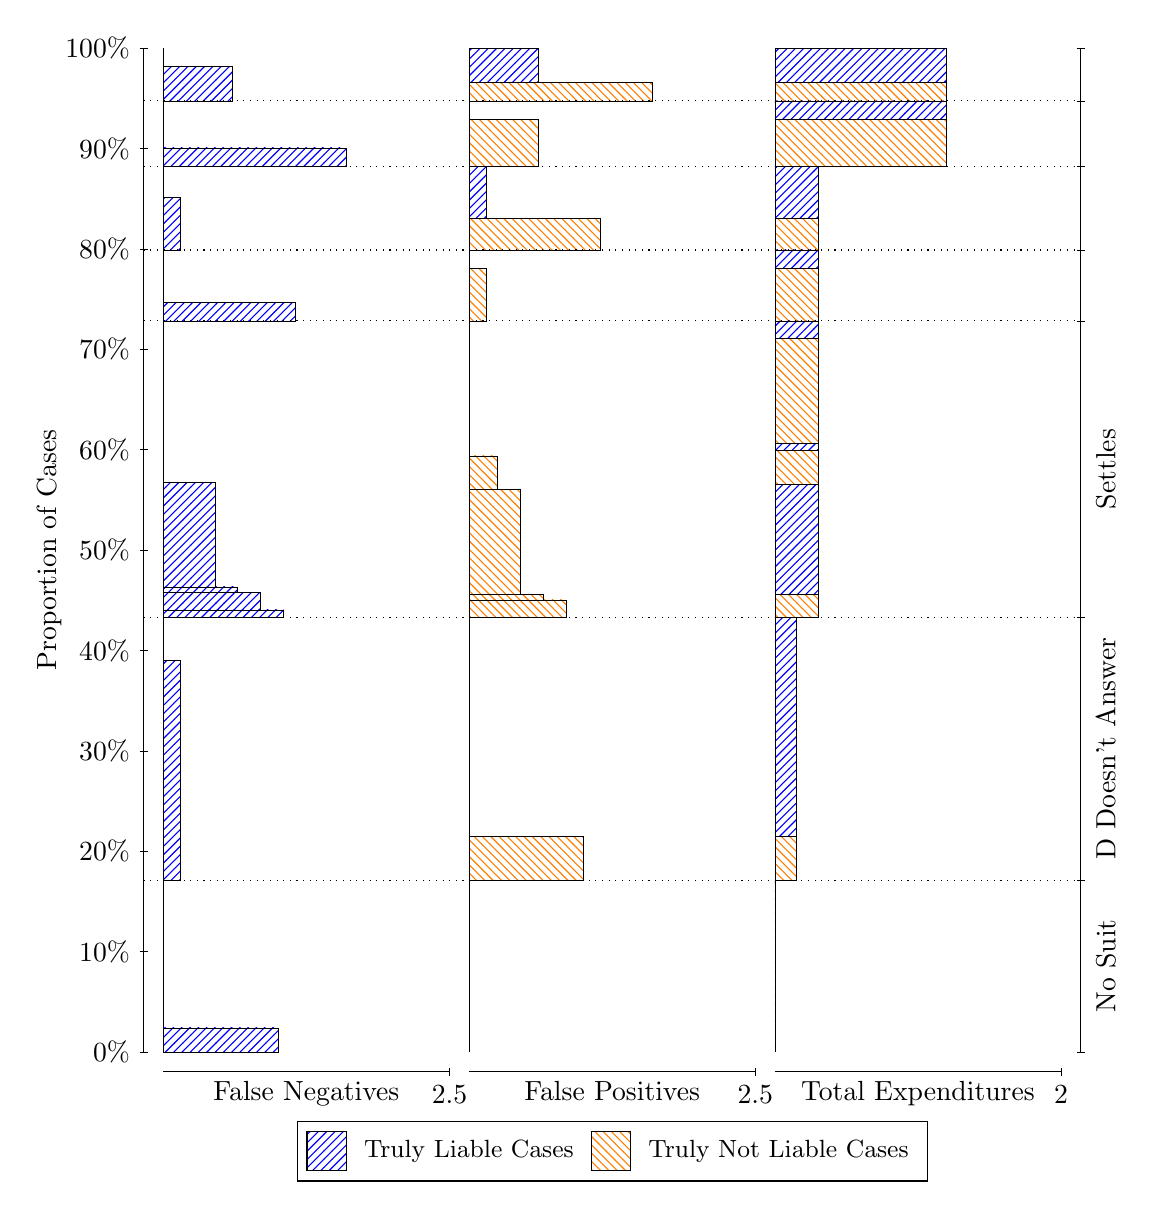
\begin{tikzpicture}
\draw[black, very thin] (1.5,1.75) -- (1.5,14.5);
\node[rotate=90, text=black, anchor=center] at (0.3, 8.125) {Proportion of Cases};
\draw[black, very thin] (1.45,1.75) -- (1.55,1.75);
\node[text=black, anchor=east] at (1.45, 1.75) {0\%};
\draw[black, very thin] (1.45,3.025) -- (1.55,3.025);
\node[text=black, anchor=east] at (1.45, 3.025) {10\%};
\draw[black, very thin] (1.45,4.3) -- (1.55,4.3);
\node[text=black, anchor=east] at (1.45, 4.3) {20\%};
\draw[black, very thin] (1.45,5.575) -- (1.55,5.575);
\node[text=black, anchor=east] at (1.45, 5.575) {30\%};
\draw[black, very thin] (1.45,6.85) -- (1.55,6.85);
\node[text=black, anchor=east] at (1.45, 6.85) {40\%};
\draw[black, very thin] (1.45,8.125) -- (1.55,8.125);
\node[text=black, anchor=east] at (1.45, 8.125) {50\%};
\draw[black, very thin] (1.45,9.4) -- (1.55,9.4);
\node[text=black, anchor=east] at (1.45, 9.4) {60\%};
\draw[black, very thin] (1.45,10.675) -- (1.55,10.675);
\node[text=black, anchor=east] at (1.45, 10.675) {70\%};
\draw[black, very thin] (1.45,11.95) -- (1.55,11.95);
\node[text=black, anchor=east] at (1.45, 11.95) {80\%};
\draw[black, very thin] (1.45,13.225) -- (1.55,13.225);
\node[text=black, anchor=east] at (1.45, 13.225) {90\%};
\draw[black, very thin] (1.45,14.5) -- (1.55,14.5);
\node[text=black, anchor=east] at (1.45, 14.5) {100\%};

\draw[black, very thin] (13.4,1.75) -- (13.4,14.5);
\draw[black, very thin] (13.35,1.75) -- (13.45,1.75);
\node[anchor=west] at (13.35, 1.75) {};
\draw[black, very thin] (13.35,3.9334) -- (13.45,3.9334);
\node[anchor=west] at (13.35, 3.9334) {};
\draw[black, very thin] (13.35,7.2711) -- (13.45,7.2711);
\node[anchor=west] at (13.35, 7.2711) {};
\draw[black, very thin] (13.35,11.034) -- (13.45,11.034);
\node[anchor=west] at (13.35, 11.034) {};
\draw[black, very thin] (13.35,11.935) -- (13.45,11.935);
\node[anchor=west] at (13.35, 11.935) {};
\draw[black, very thin] (13.35,12.998) -- (13.45,12.998);
\node[anchor=west] at (13.35, 12.998) {};
\draw[black, very thin] (13.35,13.83) -- (13.45,13.83);
\node[anchor=west] at (13.35, 13.83) {};
\draw[black, very thin] (13.35,14.5) -- (13.45,14.5);
\node[anchor=west] at (13.35, 14.5) {};

\draw[black, very thin, pattern color=blue, pattern=north east lines] (1.75,1.75) rectangle (3.2033,2.0553);
\draw[black, very thin, pattern color=orange, pattern=north west lines] (1.75,2.0553) rectangle (1.75,3.9334);
\draw[black, very thin, pattern color=blue, pattern=north east lines] (1.75,3.9334) rectangle (1.968,6.7205);
\draw[black, very thin, pattern color=orange, pattern=north west lines] (1.75,6.7205) rectangle (1.75,7.2711);
\draw[black, very thin, pattern color=blue, pattern=north east lines] (1.75,7.2711) rectangle (3.276,7.3653);
\draw[black, very thin, pattern color=blue, pattern=north east lines] (1.75,7.3653) rectangle (2.9853,7.5859);
\draw[black, very thin, pattern color=blue, pattern=north east lines] (1.75,7.5859) rectangle (2.6947,7.6554);
\draw[black, very thin, pattern color=blue, pattern=north east lines] (1.75,7.6554) rectangle (2.404,8.9864);
\draw[black, very thin, pattern color=orange, pattern=north west lines] (1.75,8.9864) rectangle (1.75,11.034);
\draw[black, very thin, pattern color=blue, pattern=north east lines] (1.75,11.034) rectangle (3.4213,11.265);
\draw[black, very thin, pattern color=orange, pattern=north west lines] (1.75,11.265) rectangle (1.75,11.935);
\draw[black, very thin, pattern color=blue, pattern=north east lines] (1.75,11.935) rectangle (1.968,12.601);
\draw[black, very thin, pattern color=orange, pattern=north west lines] (1.75,12.601) rectangle (1.75,12.998);
\draw[black, very thin, pattern color=blue, pattern=north east lines] (1.75,12.998) rectangle (4.0753,13.233);
\draw[black, very thin, pattern color=orange, pattern=north west lines] (1.75,13.233) rectangle (1.75,13.83);
\draw[black, very thin, pattern color=blue, pattern=north east lines] (1.75,13.83) rectangle (2.622,14.266);
\draw[black, very thin, pattern color=orange, pattern=north west lines] (1.75,14.266) rectangle (1.75,14.5);
\draw[black, very thin, pattern color=orange, pattern=north west lines] (5.6333,1.75) rectangle (5.6333,3.6281);
\draw[black, very thin, pattern color=blue, pattern=north east lines] (5.6333,3.6281) rectangle (5.6333,3.9334);
\draw[black, very thin, pattern color=orange, pattern=north west lines] (5.6333,3.9334) rectangle (7.0867,4.484);
\draw[black, very thin, pattern color=blue, pattern=north east lines] (5.6333,4.484) rectangle (5.6333,7.2711);
\draw[black, very thin, pattern color=orange, pattern=north west lines] (5.6333,7.2711) rectangle (6.8687,7.4916);
\draw[black, very thin, pattern color=orange, pattern=north west lines] (5.6333,7.4916) rectangle (6.578,7.5611);
\draw[black, very thin, pattern color=orange, pattern=north west lines] (5.6333,7.5611) rectangle (6.2873,8.8922);
\draw[black, very thin, pattern color=orange, pattern=north west lines] (5.6333,8.8922) rectangle (5.9967,9.3189);
\draw[black, very thin, pattern color=blue, pattern=north east lines] (5.6333,9.3189) rectangle (5.6333,11.034);
\draw[black, very thin, pattern color=orange, pattern=north west lines] (5.6333,11.034) rectangle (5.8513,11.704);
\draw[black, very thin, pattern color=blue, pattern=north east lines] (5.6333,11.704) rectangle (5.6333,11.935);
\draw[black, very thin, pattern color=orange, pattern=north west lines] (5.6333,11.935) rectangle (7.3047,12.332);
\draw[black, very thin, pattern color=blue, pattern=north east lines] (5.6333,12.332) rectangle (5.8513,12.998);
\draw[black, very thin, pattern color=orange, pattern=north west lines] (5.6333,12.998) rectangle (6.5053,13.595);
\draw[black, very thin, pattern color=blue, pattern=north east lines] (5.6333,13.595) rectangle (5.6333,13.83);
\draw[black, very thin, pattern color=orange, pattern=north west lines] (5.6333,13.83) rectangle (7.9587,14.064);
\draw[black, very thin, pattern color=blue, pattern=north east lines] (5.6333,14.064) rectangle (6.5053,14.5);
\draw[black, very thin, pattern color=orange, pattern=north west lines] (9.5167,1.75) rectangle (9.5167,3.6281);
\draw[black, very thin, pattern color=blue, pattern=north east lines] (9.5167,3.6281) rectangle (9.5167,3.9334);
\draw[black, very thin, pattern color=orange, pattern=north west lines] (9.5167,3.9334) rectangle (9.7892,4.484);
\draw[black, very thin, pattern color=blue, pattern=north east lines] (9.5167,4.484) rectangle (9.7892,7.2711);
\draw[black, very thin, pattern color=orange, pattern=north west lines] (9.5167,7.2711) rectangle (10.062,7.5611);
\draw[black, very thin, pattern color=blue, pattern=north east lines] (9.5167,7.5611) rectangle (10.062,8.9616);
\draw[black, very thin, pattern color=orange, pattern=north west lines] (9.5167,8.9616) rectangle (10.062,9.3884);
\draw[black, very thin, pattern color=blue, pattern=north east lines] (9.5167,9.3884) rectangle (10.062,9.4826);
\draw[black, very thin, pattern color=orange, pattern=north west lines] (9.5167,9.4826) rectangle (10.062,10.814);
\draw[black, very thin, pattern color=blue, pattern=north east lines] (9.5167,10.814) rectangle (10.062,11.034);
\draw[black, very thin, pattern color=orange, pattern=north west lines] (9.5167,11.034) rectangle (10.062,11.704);
\draw[black, very thin, pattern color=blue, pattern=north east lines] (9.5167,11.704) rectangle (10.062,11.935);
\draw[black, very thin, pattern color=orange, pattern=north west lines] (9.5167,11.935) rectangle (10.062,12.332);
\draw[black, very thin, pattern color=blue, pattern=north east lines] (9.5167,12.332) rectangle (10.062,12.998);
\draw[black, very thin, pattern color=orange, pattern=north west lines] (9.5167,12.998) rectangle (11.697,13.595);
\draw[black, very thin, pattern color=blue, pattern=north east lines] (9.5167,13.595) rectangle (11.697,13.83);
\draw[black, very thin, pattern color=orange, pattern=north west lines] (9.5167,13.83) rectangle (11.697,14.064);
\draw[black, very thin, pattern color=blue, pattern=north east lines] (9.5167,14.064) rectangle (11.697,14.5);
\draw[black, dotted] (1.5,3.9334) -- (13.4,3.9334);
\draw[black, dotted] (1.5,7.2711) -- (13.4,7.2711);
\draw[black, dotted] (1.5,11.034) -- (13.4,11.034);
\draw[black, dotted] (1.5,11.935) -- (13.4,11.935);
\draw[black, dotted] (1.5,12.998) -- (13.4,12.998);
\draw[black, dotted] (1.5,13.83) -- (13.4,13.83);
\draw[black, very thin] (1.75,1.5) -- (5.3833,1.5);
\node[text=black, anchor=north] at (3.5667, 1.5) {False Negatives};
\draw[black, very thin] (5.3833,1.45) -- (5.3833,1.55);
\node[text=black, anchor=north] at (5.3833, 1.45) {2.5};

\draw[black, very thin] (5.6333,1.5) -- (9.2667,1.5);
\node[text=black, anchor=north] at (7.45, 1.5) {False Positives};
\draw[black, very thin] (9.2667,1.45) -- (9.2667,1.55);
\node[text=black, anchor=north] at (9.2667, 1.45) {2.5};

\draw[black, very thin] (9.5167,1.5) -- (13.15,1.5);
\node[text=black, anchor=north] at (11.333, 1.5) {Total Expenditures};
\draw[black, very thin] (13.15,1.45) -- (13.15,1.55);
\node[text=black, anchor=north] at (13.15, 1.45) {2};

\node[text=black, centered, rotate=90] at (13.72, 2.8417) {No Suit};
\node[text=black, centered, rotate=90] at (13.72, 5.6022) {D Doesn't Answer};
\node[text=black, centered, rotate=90] at (13.72, 9.1527) {Settles};





\draw (7.449999999999999,1.5) node[draw=none] (baseCoordinate) {};
\begin{scope}[align=center]
        \matrix[scale=0.5, draw=black, below=0.5cm of baseCoordinate, nodes={draw}, column sep=0.1cm]{
            \node[rectangle, draw, minimum width=0.5cm, minimum height=0.5cm, pattern color=blue, pattern=north east lines] {}; &
            \node[draw=none, font=\small, text=black] (B) {Truly Liable Cases}; &
            \node[rectangle, draw, minimum width=0.5cm, minimum height=0.5cm, pattern color=orange, pattern=north west lines] {}; &
            \node[draw=none, font=\small, text=black] (B) {Truly Not Liable Cases}; \\
            };
\end{scope}

\end{tikzpicture}
\end{document}